\documentclass[lecture.tex]{subfiles}

\begin{document}

\exercice{Université Rennes 1 - L. Blanchard}
%\video{https://youtu.be/blablabla}
\enonce{rdm-0027}{}

La poutre de longueur $2L$ est encastrée en $x=0$. La poutre est soumise à :
\begin{itemize}[label =\ding{110},font =\tiny]
  \item une force ponctuelle $F$ suivant $\vec{y}$ en $x=2L$
  \item une force ponctuelle $2F$ suivant $\vec{y}$ en $x=L$
  \item un couple ponctuel $C$ suivant $\vec{z}$ en $x=L$
\end{itemize}

La section constante de la poutre est de hauteur (suivant $\vec{y}$) $h$ et de largeur (suivant $\vec{z}$) $b$. La poutre est en alliage d'aluminium de module d'élasticité $E=70 \ GPa$ et de limite élastique $R_{e}=320 \ MPa$. L'accélération de la pesanteur n'est pas prise en compte.

\medskip

On donne

\begin{center}
  \begin{tabular}{|l|l|l|l|l|}
    \hline\vspace{2pt}
    L = 400 \ mm &
    F = 400 \ N &
    C = 400 \ N.m &
    b = 400 \ mm &
    h = 400 \ mm \\
    \hline
  \end{tabular}
\end{center}

\begin{center}
  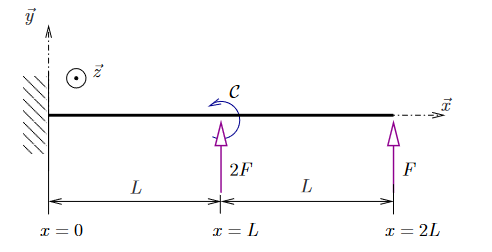
\includegraphics[scale=0.7]{figA0027.png}
\end{center}

\begin{enumerate}
  \item Calculez numériquement l'action exercée par l'encastrement sur la poutre.
  \item Calculez analytiquement, puis numériquement, les expressions de l'effort tranchant $T(x)$ suivant la  direction $\vec{y}$ et du moment fléchissant $M(x)$ suivant la direction $\vec{z}$.\par
  Tracez précisement les graphes de ces fonctions en précisant des valeurs numériques sur les axes.
  \item Calculer la contrainte maximum de tension (traction-compression). Quel(s) point(s) subit (subissent) cette contrainte en traction, en compression? Est-on encore dans le domaine élastique?
  \item Déterminer la flèche $v(x)$. Précisez les conditions que doit respecter $v(x)$.
\end{enumerate}

\finenonce{rdm-0027}
\finexercice


\end{document}
